\section{Stationäre Strömungsanalyse}
% Anwendung: Auslegung eines Erdungssystems
% die Elektrische Leitfähigkeit relevant und nicht die elektrische Permittivität (= Unterschied zu vorherigen Analyse) sonst "Copy-Paste"

\begin{tabular}[h]{ C{.2\linewidth} P{.3\linewidth} P{.4\linewidth} }
	{\vspace{0pt}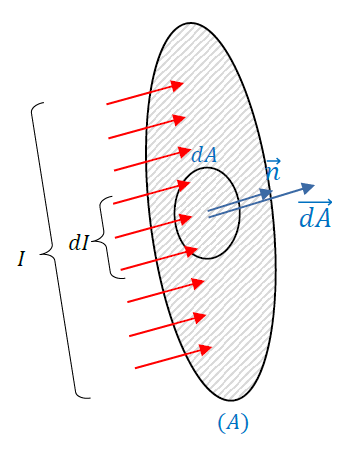
\includegraphics[width = 0.15\textwidth]{images/ElStromdichte}} & \textbf{Elektrische Stromdichte} \[ \vec{J} = \dfrac{dI}{dA}\cdot \vec{n}\qquad [\vec{J}] = \dfrac{A}{m^2} \] \[I = \iint\limits_{(A)}\vec{J}\cdot\vec{dA} \] & {\scriptsize \textcolor{blue}{\textbf{dA} - eine kleine zur Stromrichtung senkrechte Fläche \newline $\vec{\textbf{n}}$ - der senkrechte Einheitsvektor der Fläche dA \newline 
			\textbf{dI}- der durch die Fläche dA fliessende Teil des Stromes I}} \\
	& \textbf{Kontinuitätsgleichung:} \newline
	\[ I = -\dfrac{dQ}{dt} = -\dfrac{d}{dt}\iiint\limits_{(V)}\varrho\cdot dV = -\iiint\limits_{(V)}\dfrac{d\varrho}{dt}\cdot dV \] \newline \[ \varoiint\limits_{(A)}\vec{J}\cdot\vec{dA} = -\iiint\limits_{(V)}\dfrac{d\varrho}{dt}\cdot dV \] 
	{\scriptsize{In der stationären Strömungsanalyse:}} \newline 
	\[ \varoiint\limits_{(A)}\vec{J}\cdot\vec{dA} = 0\] & \\
	{\vspace{0pt}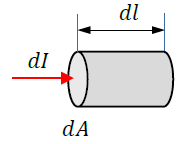
\includegraphics[width = 0.15\textwidth]{images/OhmschesGesetz}}& \textbf{Ohmsches Gesetz:} & \\
	
\end{tabular}

Der gesamte Strom durch die Fläche A




\[ \varoiint\limits_{(A)}\vec{J}\cdot\vec{dA} = -\iiint\limits_{(V)}\dfrac{d\varrho}{dt}\cdot dV \] 
und stationär sieht diese Gleichung folgendermassen aus:
\[ \varoiint\limits_{(A)}\vec{J}\cdot\vec{dA} = 0\]

\textbf{Ohmsches Gesetz:}
\[ R = \varrho\cdot\dfrac{l}{A}\]
\[ \sigma = \dfrac{1}{\varrho}\]
\[ G = \sigma\cdot\dfrac{A}{l} \]
\clearpage
\pagebreak